%%%%%%%%%%%%%%%%%%%%%%%%%%%%%%%%%%%%%%%%%%%%%%%%%%%%%%%%%%%%%%%%%%%%
%% I, the copyright holder of this work, release this work into the
%% public domain. This applies worldwide. In some countries this may
%% not be legally possible; if so: I grant anyone the right to use
%% this work for any purpose, without any conditions, unless such
%% conditions are required by law.
%%%%%%%%%%%%%%%%%%%%%%%%%%%%%%%%%%%%%%%%%%%%%%%%%%%%%%%%%%%%%%%%%%%%

\documentclass{beamer}
\usetheme[faculty=fi]{fibeamer}
\usepackage[utf8]{inputenc}
\usepackage[
  main=english, %% By using `czech` or `slovak` as the main locale
                %% instead of `english`, you can typeset the
                %% presentation in either Czech or Slovak,
                %% respectively.
  czech, slovak %% The additional keys allow foreign texts to be
]{babel}        %% typeset as follows:
%%
%%   \begin{otherlanguage}{czech}   ... \end{otherlanguage}
%%   \begin{otherlanguage}{slovak}  ... \end{otherlanguage}
%%
%% These macros specify information about the presentation
\title{Adversarial Attacks in Image Captchas} %% that will be typeset on the
\subtitle{Team Members} %% title page.
\author{Adhithya S. 03\\Janaki Keerthi  26\\Jayasoorya Jithendra  28\\Jessal V.A.  29}



%% These additional packages are used within the document:
\usepackage{ragged2e}  % `\justifying` text
\usepackage{booktabs}  % Tables
\usepackage{tabularx}
\usepackage{tikz}      % Diagrams
\usetikzlibrary{calc, shapes, backgrounds}
\usepackage{amsmath, amssymb}
\usepackage{url}       % `\url`s
\usepackage{listings}  % Code listings
\frenchspacing
\begin{document}
  \frame{\maketitle}
 % \tableofcontents
  \AtBeginSection[]{% Print an outline at the beginning of sections
    \begin{frame}<beamer>
      %\frametitle{Outline for Section \thesection}
      \tableofcontents[currentsection]
    \end{frame}}

  \begin{darkframes}
    \section{Problem Statement}
    \begin{frame}{Problem Statement}
     % \begin{tikzpicture}[overlay,remember picture]
     %   \node[anchor=south east,xshift=-30pt,yshift=35pt]
     %     at (current page.south east) {
     %       
\includegraphics[width=35mm]{resources/jabberwocky-dark}
     %     };
     % \end{tikzpicture}%
      To perform adversarial attacks on Image captchas to prevent bots from automating captcha tests.\\
      
    \end{frame}
    
    \section{Introduction}
    
    \subsection{Why Adversarial Attacks work?}
    \begin{frame}{Why Adversarial Attacks work?}
    
    
        Modern hardware manipulate images as 8 bit values.\\\bigskip
        Modern Neural Networks manipulate data in 32 bit floating point numbers.\\\bigskip
        Thus Adversarial Attacks manipulate the data such that the main 8 bits are unchanged, by modifying the remaining 24 bits.\\\bigskip
        

    \end{frame}

    \subsection{Where Modern Neural Networks fail?}
    \begin{frame}{Where Modern Neural Networks fail?}
    
    
        Neural Networks perform linear transformation to the matrices.\\\bigskip
        Additions of dropout, pre-training, and model averaging do not improve the model’s vulnerability to adversarial examples.\\\bigskip
        Convolutional neural networks approximates Perceptual distance as Euclidean distance.\\\bigskip
        This resemblance is clearly flawed if images that have an
        immeasurably small perceptual distance correspond to completely different classes in the network’s representation.
        

    \end{frame}

    \section{Fast Gradient Sign Methods}
    \subsection{The Linear Explanation of Adversarial Examples}
    \begin{frame}{The Linear Explanation of Adversarial Examples}
        The precision of the features is limited.\\\bigskip
        It is not rational for the classifier to respond differently to an input x than to an adversarial input $ x~ = x + \eta$  if every element of the perturbation $\eta$ is smaller than the precision of the features\\\bigskip
        Precision of the features is about (1/256) $\approx$ (0.03).
        Thus for $\eta \leq (0.03)$ the adversarial input should act similiar to the original input.\\\bigskip
        
        Thus effectively the transformation becomes:\\
        \centerline{$ W^{T}*\widetilde{x} = W^{T}*x + W^{T}*\eta $}
    \end{frame}

    \subsection{Linear Perturbation of Non-Linear Models}
        
    
    \begin{frame}{Linear Perturbation of Non-Linear Models}
    \framesubtitle{Introduction}
        
        Let $\theta$ be the parameters of a model, x the input to the model, y the targets associated with x and $J(\theta,x, y)$ be the cost used to train the neural network.
    
        \centerline{$\eta = \epsilon . sign(\nabla_{x}J(\theta,x, y))$}
        \begin{center}
        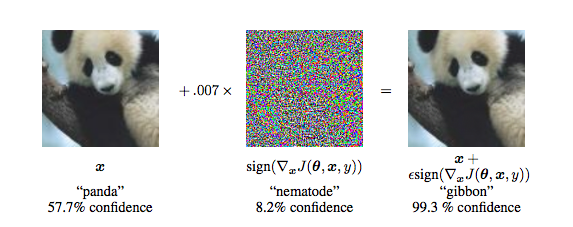
\includegraphics[width=3.5in]{panda.png}
        \end{center}
    
    \end{frame}
    
    \subsection{One shot Fast Gradient Sign Method}
    \begin{frame}{Fast Gradient Sign Method}
        
        FGSM computes an adversarial image by adding a pixel-wide perturbation of magnitude in the direction of the gradient. This perturbation is computed with a single step, thus is very efficient in terms of computation time.\\\bigskip
        
        \centerline{$X^{adv} = x + \epsilon . sign(\nabla_{x}J(x, y_{true}))$}\\\bigskip
        
        \begin{flushleft}
        where,\\
        X : is the clean input\\
        $X^{adv}$ : is the perturbed adversarial example.\\
        J : is the classifier's loss function.\\
        $y_{true}$ : is the true label for the input x.\\
        \end{flushleft}
        
    \end{frame}

    \subsection{Targeted and Iterative Fast Gradient Sign Method}
    \begin{frame}{Targeted and Iterative Fast Gradient Sign Method}
        
        \textbf{Targeted Fast Gradient Sign Method}
        Similarly to the FGSM, in this method a gradient step is computed, but in this case in the direction of the negative gradient with respect to the target class:\\\bigskip
        
        \centerline{$X^{adv} = x - \epsilon . sign(\nabla_{x}J(x, y_{target}))$}\\\bigskip
        
        
        \textbf{Iterative Fast Gradient Sign Method}
        The iterative methods take T gradient steps of magnitude 
        $ \alpha = \epsilon / T $ instead of a single step t:
        
        \centerline{$X^{adv}_{0} = X$}\\
        \centerline{$X^{adv}_{t+1} = X^{adv}_{t} + + \alpha . sign(\nabla_{x}J(x, y_{true}))$}
        
    \end{frame}
   
    \subsection{Comparison of various Fast Gradient Sign Method} 
    \begin{frame}{Comparison of various Fast Gradient Sign Method}
        
        Both one-shot methods (FGSM and T-FGSM) have lower success rates when compared to the iterative methods (I-FGSM) in white box attacks.\\\bigskip
        
        When it comes to black box attacks the basic single-shot methods turn out to be more effective.\\\bigskip
        
        The most likely explanation for this is that the iterative methods tend to overfit to a particular mode.
        
    \end{frame}
    
    

    \section{Bibliography}
    %\begin{frame}[label=citations]{Citations}
    %\end{frame}

    \begin{frame}[label=bibliography]{Bibliography}
      \begin{thebibliography}{9}
        \bibitem{knuth84}
            Ian J. Goodfellow, Jonathon Shlens & Christian Szegedy - Explaining and harnessing Adversarial Examples,2015
        \bibitem{lamport94}
            Gamaleldin F. Elsayed, Ian Goodfellow, Jascha Sohl-Dickstein - Adversarial Reprogramming of Neural Networks,2018
        \bibitem{MG94}
           F. Tramèr et al. “Ensemble Adversarial Training: Attacks and Defenses”. In: ArXiv e-prints
(May 2017).
        
      \end{thebibliography}
    \end{frame}

  \end{darkframes}


\end{document}
